\documentclass{article}
\usepackage{graphicx} % Required for inserting images
\usepackage{amsmath}
\usepackage{mathtools}
\usepackage{hyperref}
\usepackage{color,soul}
\usepackage{xcolor}
\usepackage{hyperref}
\hypersetup{
    colorlinks=true,
    linkcolor=blue,
    filecolor=magenta,      
    urlcolor=cyan,
    pdftitle={Overleaf Example},
    pdfpagemode=FullScreen,
    }

\title{report}
\author{Siddhartha }
\date{June 2024}

\begin{document}

\maketitle
\tableofcontents
\newpage
\section{MOSFET Model}
\subsection*{Constants}
\begin{align}    
    n_i &= 10^{10}/cm^3 \\
    \epsilon_{ox} &= 3.9\times8.854\times10^{-14} F/cm  \\
    \epsilon_s &= 11.9\times8.854\times1e-14 F/cm  
\end{align}

\subsection*{Variable Parameters}
\begin{align}
    N_A &= 10^{15} /cm^{3} \\
    t_{ox} &= 2\times10^{-5} cm \\
    V_{FB} &= 1.035  V \\
    q &= 1.60217663 \times 10^{-19}  C \\
    W &= 0.22 \times 10^{-4} cm \\
    L &= 4  \times 10^{-4}  cm \\
    V_{BS} &= -10 V \\
    \mu_n  &= 1340 cm^2/(V.s) 
\end{align}
\subsection*{Calculations}
\begin{align}
    C_{ox} &= \frac{\epsilon_{ox}}{t_{ox}} \\
    \phi_B &= 0.0258\log(N_A/n_i)\\
    V_{th} &= V_{FB} + 2 \phi_{B} + \frac{\sqrt{2q N_A \epsilon_s 2 \phi_B}}{C_{ox}}  V  \\
    \gamma &= \frac{\sqrt{2\times\epsilon_s q N_A}}{C_{ox}} \\
    \alpha &= 1 + \gamma/(2\sqrt{2\phi_B-V_{BS}}) 
\end{align}
\subsection*{Level-3 Model}

\begin{equation}
    V_{DSat} = (V_{GS} - V_{th})/\alpha 
\end{equation}
\begin{equation}
    I_{DS} = \begin{cases}
        \frac{\mu_n C_{ox} W}{2L} (V_{GS}-V_{th}) \left[ 2V_{DS} - \frac{V_{DS}^2}{V_{DSat}}\right], & \text{ if } V_{DS}\leq V_{DSat} \\
        \frac{\mu_n C_{ox} W}{2L} (V_{GS}-V_{th}) V_{DSat}, & \text { if } V_{DS} \geq V_{DSat}
    \end{cases} 
\end{equation}

\subsection*{Simulations}

\begin{align}
        V_{DSeff} &= V_{DS} -  \frac{1}{2}(V_{DS}-V_{DSat}+\sqrt{(V_{DS}-V_{DSat})^2 + \Delta^2}) \\
        V_{DSeff} &= \begin{cases}
        V_{DS}, & \text{ if } V_{DS}\leq V_{DSat} \\
        V_{DSat}, & \text { if } V_{DS} \geq V_{DSat}
        \end{cases}
\end{align}

\begin{align} 
    \label{eq:DrainCurrent}
    I_{DS} &= \frac{\mu_n C_{ox} W}{2L}(V_{GS}-V_{th}) \left(2V_{DSeff} - \frac{V_{DSeff}^2}{V_{DSat}}\right)
\end{align}

\newpage

\subsection*{Plot-digitizer}
\href{https://plotdigitizer.com/app}{Plot digitizer} app is used to digitize the plot given in the paper and the data obtained is used to calculate the gain factor.  
\begin{center}
        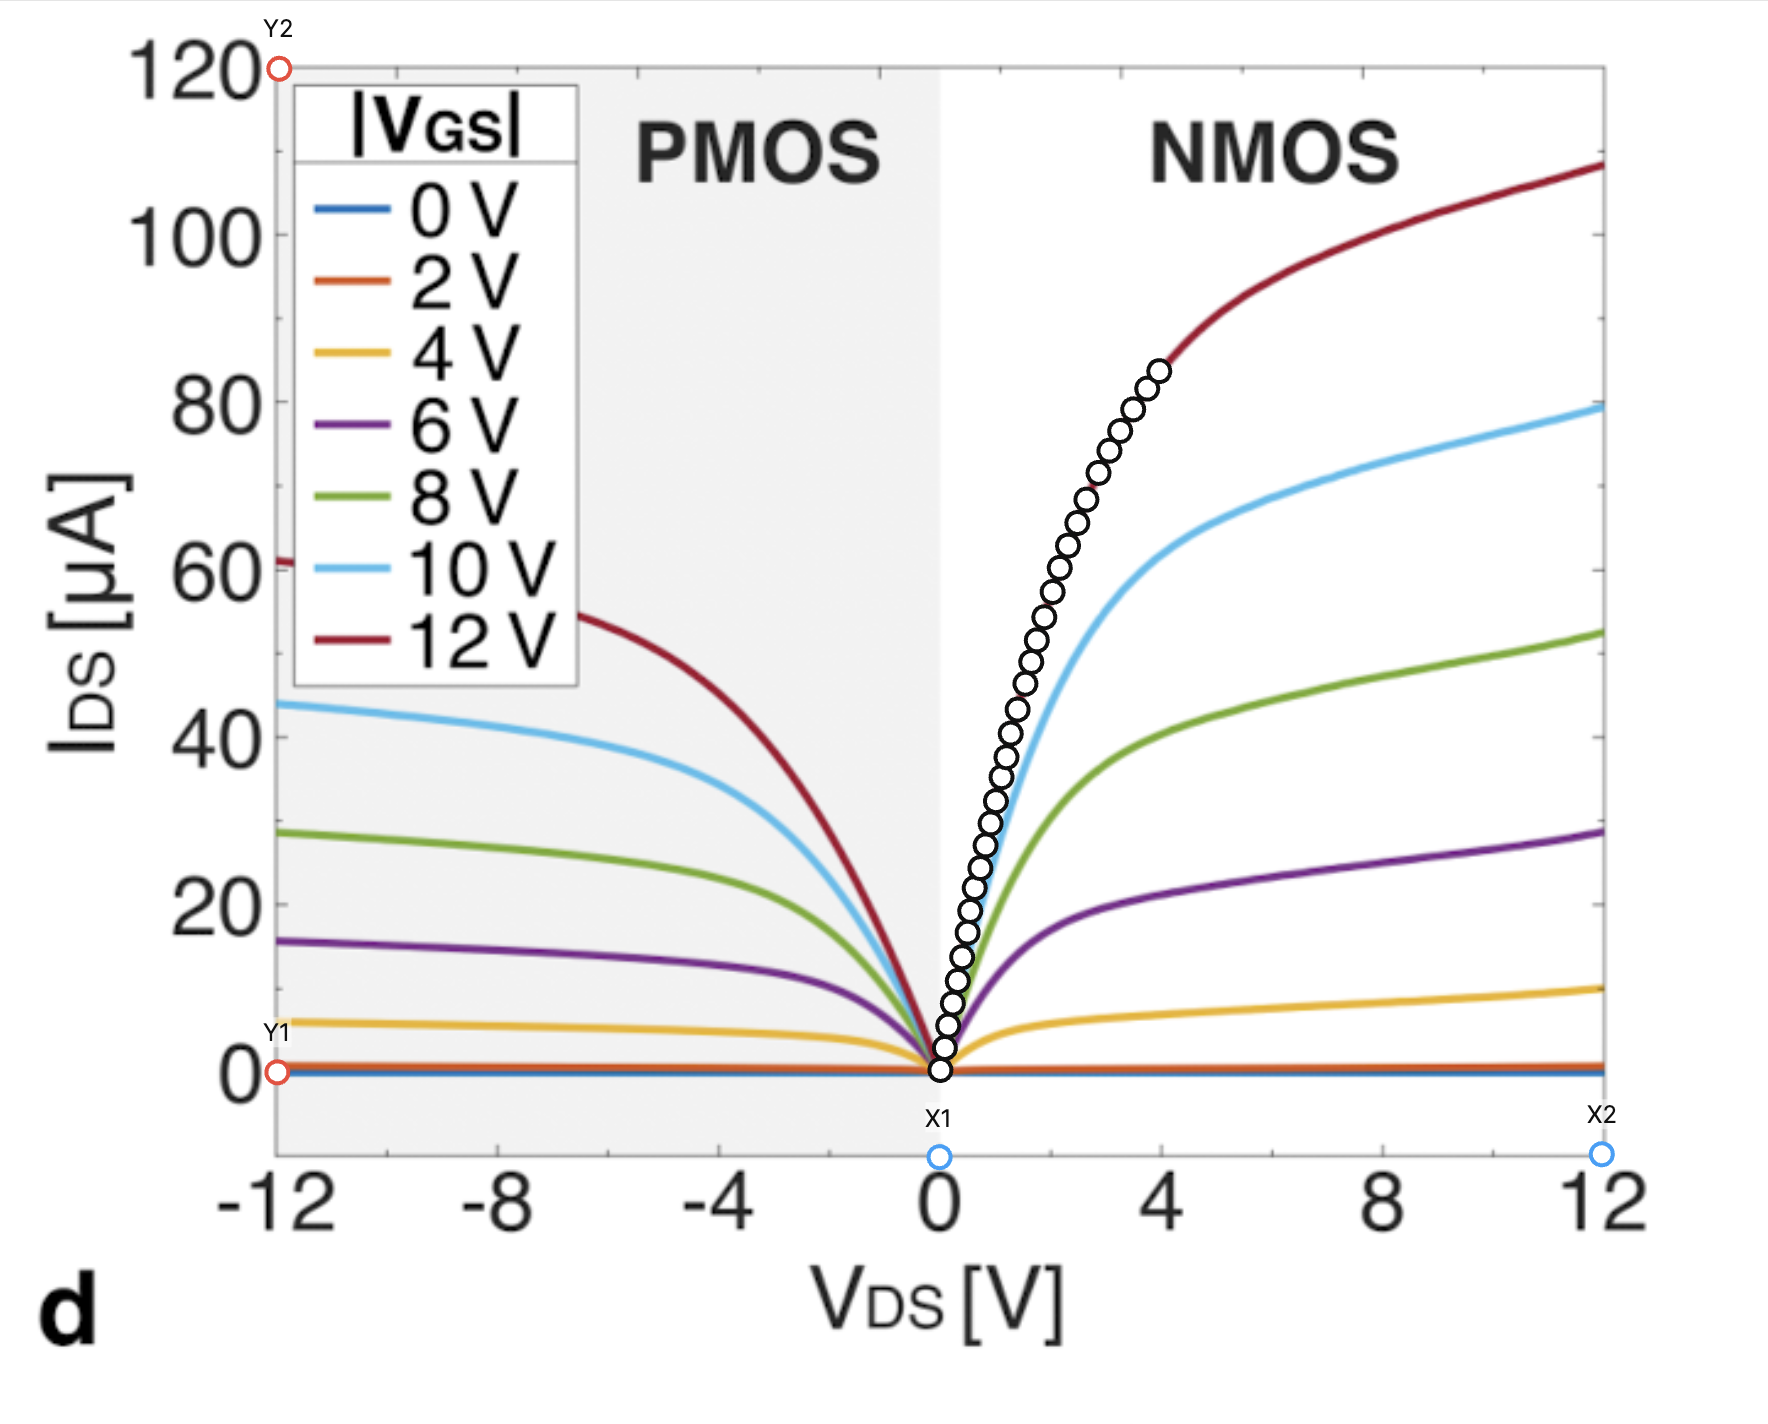
\includegraphics[scale = 0.3]{../Images/Previous/Plot-analyzer.png}        
\end{center}
    

\begin{align*}
    I_{DS}(2.05 V) &= 57.44 \mu A \\
    I_{DS}(0.01 V) &= 00.28 \mu A 
\end{align*}

In equation \ref{eq:DrainCurrent} if we assume linearity with $V_{DS}$ and neglecting the term $\frac{V_{DS}^2}{2V_{DSat}}$ the gain factor is given by the equation \ref{eq:gain-factor}. 
\begin{align}
    \label{eq:gain-factor}
    \mu C_{ox} \frac{W}{L} &= \frac{1}{V_{GS}-V_{th}}\times\frac{I_{DS}(2.05 \; V) - I_{DS}(0.01 \; V)}{2.05-0.01} \\
    \mu C_{ox} \frac{W}{L} &= \frac{1}{12-2.45}\times\frac{57.44 - 00.28}{2.05-0.01} \mu A/V^2 \\ 
    \mu C_{ox} \frac{W}{L} &= 2.93 \mu A/V^2
\end{align}
The gain factor given in the reference is $4 \mu A/V^2$ the difference may be due to the fact that the Current through channel is not a linear function of $V_{DS}$. 
\newpage
\subsection*{Comparing acquired data with level-3 model}
The Drain current ($I_{DS}$) is calculated using the level-3 model given by equation \ref{eq:DrainCurrent}, the gain factor is fixed at the value $4 \mu A/V^2$ as described in the paper. The comparison of calculated drain current and acquired drain current is shown in figure (\ref{fig:ids-comp-4}).
\begin{center}
    \label{fig:ids-comp-4}
    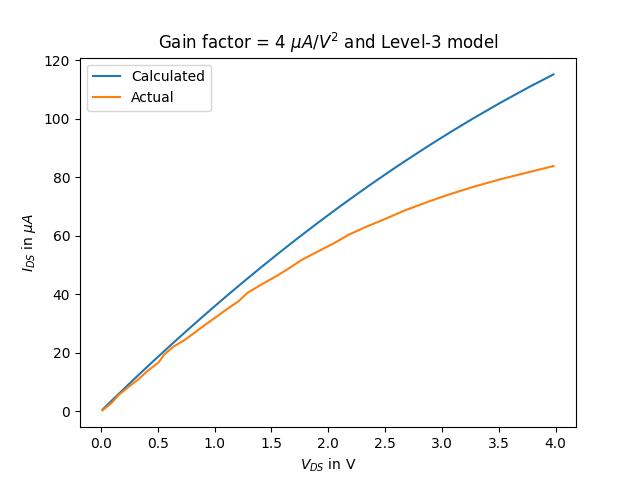
\includegraphics[scale = 0.6]{../Images/Previous/Ids-comp.png}    
\end{center}


If the gain factor is reduced to $3.5 \mu A / V^2$ the Comparison graph is as shown below in figure (\ref{fig:ids-comp-3.5}). 
\begin{center}
    \label{fig:ids-comp-3.5}
    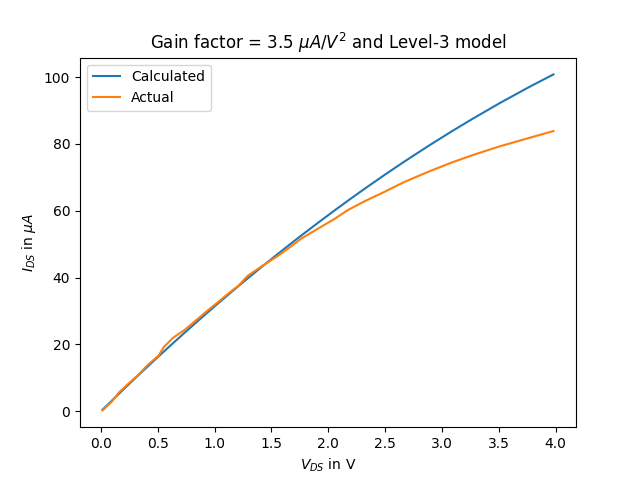
\includegraphics[scale = 0.6]{../Images/Previous/Ids-comp-3.5.png}

\end{center}
The plot of $V_{GS} = 10 V$ is digitized and compared with the model with gain factor = 3.5 V the comparison is shown in figure (\ref{fig:ids-comp-10-3.5}). The range of $V_{DS}$ considered is $0 V \to 2.5 V$ because the plot is linear in that region. 

\begin{center}
    \label{fig:ids-comp-10-3.5}
    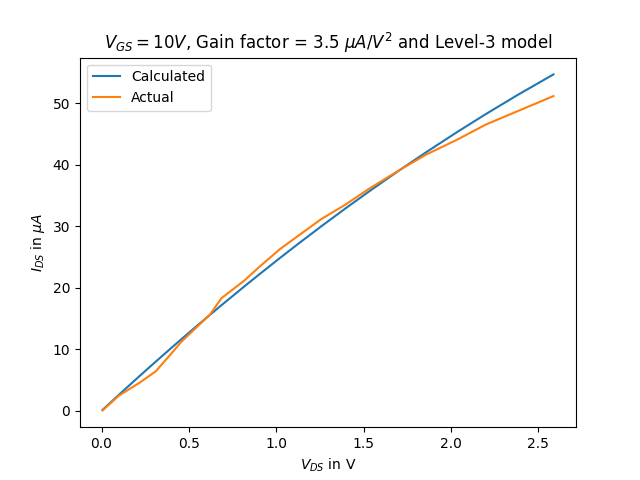
\includegraphics[scale=0.6]{../Images/Previous/Ids-comp-10-3.5.png}
\end{center}
The comparison of Calculated and acquired data for $V_{GS} = 12 V$ and for  $V_{DS}$  in range of $0 V\to 2.5 V $ is shown in figure (\ref{fig:ids-comp-12-3.5}). 
\begin{center}
    \label{fig:ids-comp-12-3.5}
    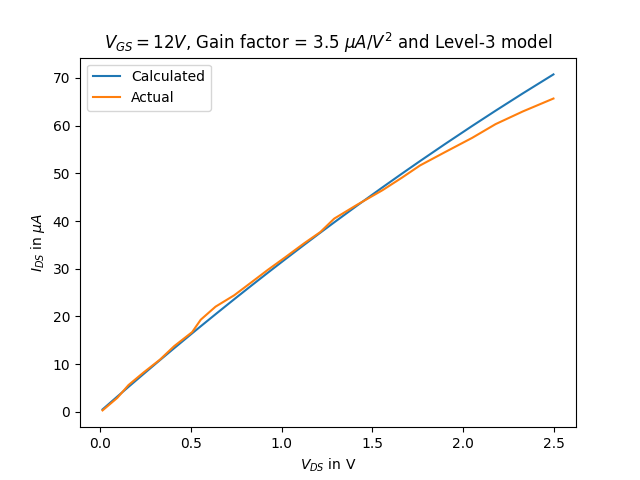
\includegraphics[scale=0.6]{../Images/Previous/Ids-comp-12-3.5.png}
\end{center}

\newpage

\subsection*{Four MOS-CAPs in parallel}

\subsection*{Model}
The data from the plot is extracted for the gate voltage values of 
\newline$4V, \; 6V, \;  8V, \; 10V, \; 12V$  and plotted in figure \ref{fig:Plot-Data-Digitized}.
\begin{center}
    \label{fig:Plot-Data-Digitized}
    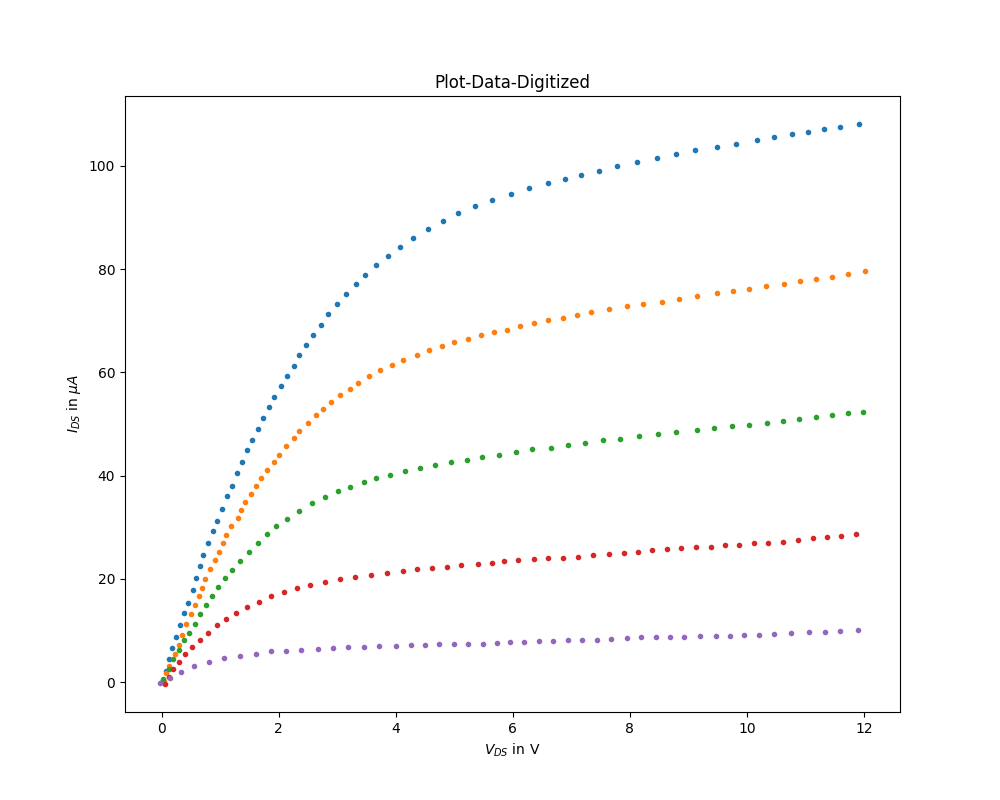
\includegraphics[scale = 0.4]{../Images/Previous/Plot-Data-Digitized.png}
\end{center}
Since, there is a small slope in saturation region the previous model is modified and the new modified model contains a new parameter $\lambda$. 
The new model is given by the equation \ref{eq:new-model}. 
\begin{equation}
    \label{eq:new-model}
    \boxed{I_{DS} =  \text{ gain } \times \alpha (V_{DSeff}V_{DSat} - \frac{V_{DSeff}^2}{2})(1+\lambda V_{DS})  }
\end{equation}

where, 
\begin{align}
    \alpha &= \text{ Level - 3 model Parameter } \\
    \text { Gain } &= \frac{\mu C_{ox} W }{L}\\
    V_{DSat} &= \frac{V_{GS} - V_{th}}{\alpha} \\
\end{align}
\newpage
\subsection*{Fit - 1}
Variable parameters to fit the model for different values of $V_{GS}$ and $V_{DS}$. 
\begin{itemize}
    \item $\alpha$ = 2.2
    \item $\text{gain}$ = 4
    \item $\lambda$ = 0.05
    \item $V_{th}$ = 2.45
\end{itemize}
\begin{center}
    \label{fig:model-fit-1}
    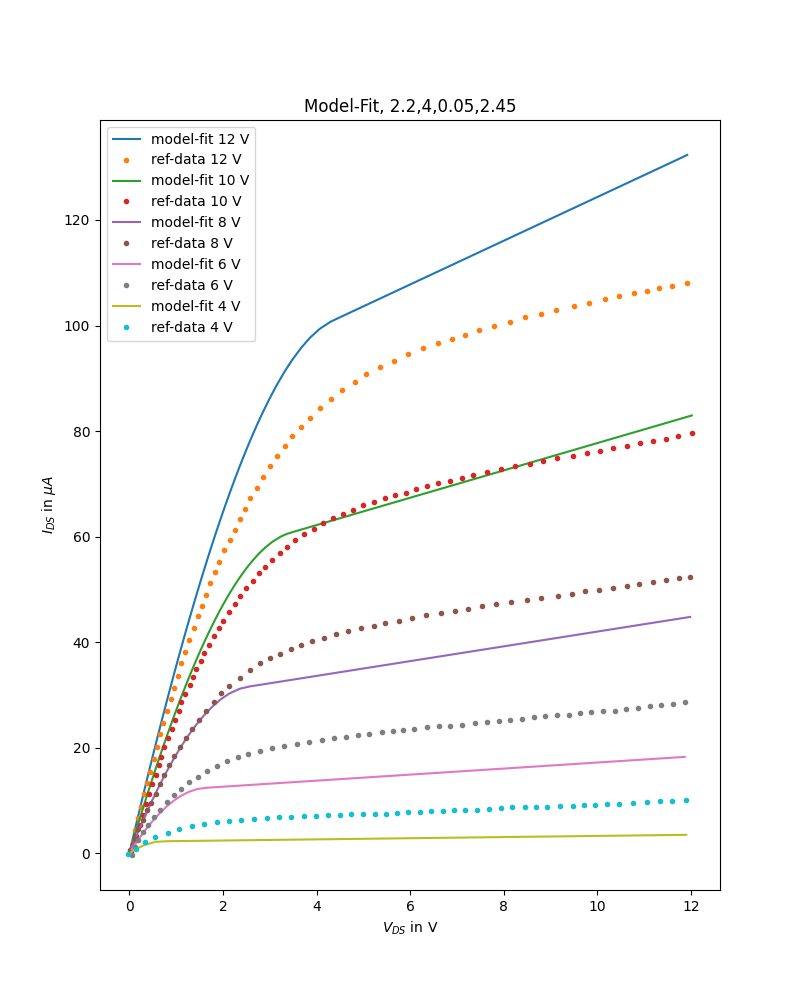
\includegraphics[scale = 0.4]{../Images/Previous/Model-Fit-2.2-4-0.05-2.45.png}
\end{center}
\newpage
\subsection*{Fit - 2}
Variable parameters to fit the model for different values of $V_{GS}$ and $V_{DS}$. 
\begin{itemize}
    \item $\alpha$ = 3
    \item $\text{gain}$ = 3
    \item $\lambda$ = 0.044
    \item $V_{th}$ = -0.2
\end{itemize}
With the parameters set the model is fit and shown in the figure \ref{fig:model-fit-2}.
\begin{center}
    \label{fig:model-fit-2}
    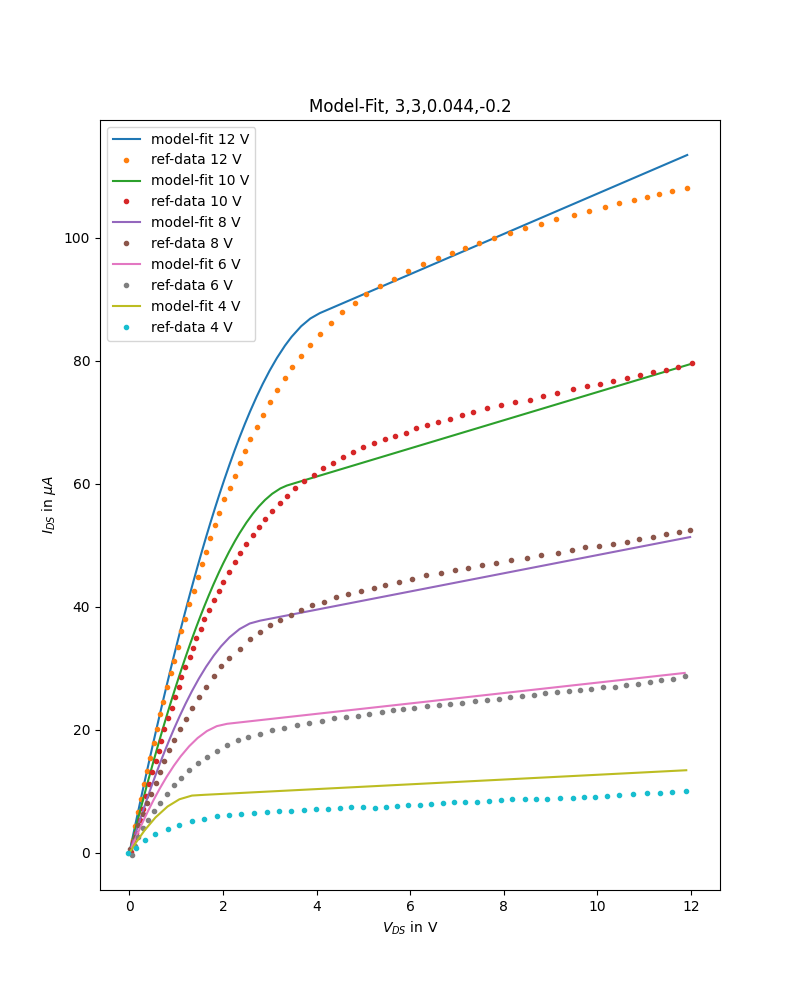
\includegraphics[scale = 0.4]{../Images/Previous/Model-Fit-3-3-0.044--0.2.png}
\end{center}
\subsubsection*{Analysis of the Fit}
\textbf{$V_{DS}< V_{DSat}$}
\begin{equation}
    I_{DS} = \text{ gain }\times \left[(V_{DS}(V_{GS}-V_{th})) - \frac{(V_{GS}-V_{th})^2}{2 \alpha}\right](1 + \lambda V_{DS})
\end{equation}
\textbf{$V_{DS}\geq V_{DSat}$}
\begin{equation}
    I_{DS} =\text{ gain }\times \frac{(V_{GS}-V_{th})^2}{2\alpha} (1 + \lambda V_{DS})
\end{equation}
\newpage
\subsection*{QUCS simulations}
There is some resistance in between source contact pad and source terminal in transistor therefore, we model a resistor in between them and similarly a resistance between drain contact pad drain terminal at transistor. The resistance is calculated as shown in equation (\ref{eq:resistance}). 
\begin{equation}
    \label{eq:resistance}
                 R = \frac{\rho L}{A} = \frac{0.085 \times 6}{2*0.22 \times10^{-4}} = 11590 \Omega
\end{equation}
The model used to simulate is as shown in the figure \ref{fig:model-1}. $I_D$ is given by equation \ref{eq:model-i-eq}. 
\begin{equation}
    \label{eq:model-i-eq}
    \boxed{I_{D} = \alpha*\text{gain}*(V_{DSeff}V_{DSat}-\frac{V_{DSeff}^2}{2})(1+\lambda V_{DSi})}
\end{equation}
the equations of $V_{DSeff}$, $V_{DSat}$ and $V_{DSi}$ are given by equation \ref{eq:model-v-eqs}
\begin{align}
    \label{eq:model-v-eqs}
    V_{GSi}   &= V_{GS} - V_{Si} \\
    V_{DSi}   &= V_{DS} - V_{Si} \\
    V_{DSat}  &= (V_{GSi} - V_{th})/\alpha \\
    V_{DSeff} &= V_{DSi} - \frac{1}{2}(V_{DSi}-V_{DSat}+\sqrt{(V_{DSi}-V_{DSat})^2+\Delta^2)}
\end{align}
The parameters are $\alpha$, gain, $V_{th}$, $\lambda$
\begin{center}
    \label{fig:model-1}
    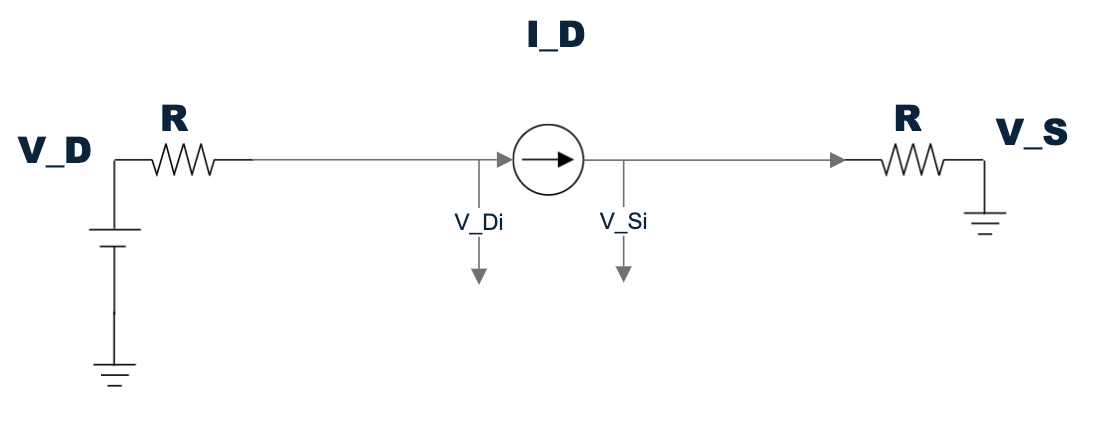
\includegraphics[scale=0.4]{../Images/Previous/model-1.png}
\end{center}
\newpage
\section{22-07-2024}
\subsection{Above threshold and sub-threshold currents}
Current equation for above threshold is given by equation (\ref{eq:Iat})
\begin{equation}
    \label{eq:Iat}
    I_{at} = \text{ gain } (\frac{V_{gt}}{\alpha} V_{dseff} - \frac{V_{dseff}^2}{2})
\end{equation}
where,
$$V_{gt} = \begin{cases}
    V_{gs} - V_{th} &\text{ if } V_{gs} - V_{th} >0\\
    0 &\text{ otherwise }
\end{cases}$$
Current equation for sub-threshold region is given by equation (\ref{eq:Ist})
\begin{equation}
    \label{eq:Ist}
    I_{st} = \frac{I_{s}I_{p}}{I_{s}+I_{p}}
\end{equation}
The equation of $I_s$ is given by equation (\ref{eq:Is})
\begin{equation}
    \label{eq:Is}
    I_s = I_o \exp{\frac{V_{gs}-V_{th}}{m V_{T}}}
\end{equation}
where, $I_{o} = I_{at}(V_{gs} = V_{th} + 3V_T)$ and $I_{p} = I_{at}(V_{gs} = V_{th} + 4V_T) $
The figure (\ref{fig:at-st}) shows the above threshold and sub-threshold currents. 
\begin{center}
    \label{fig:at-st}
    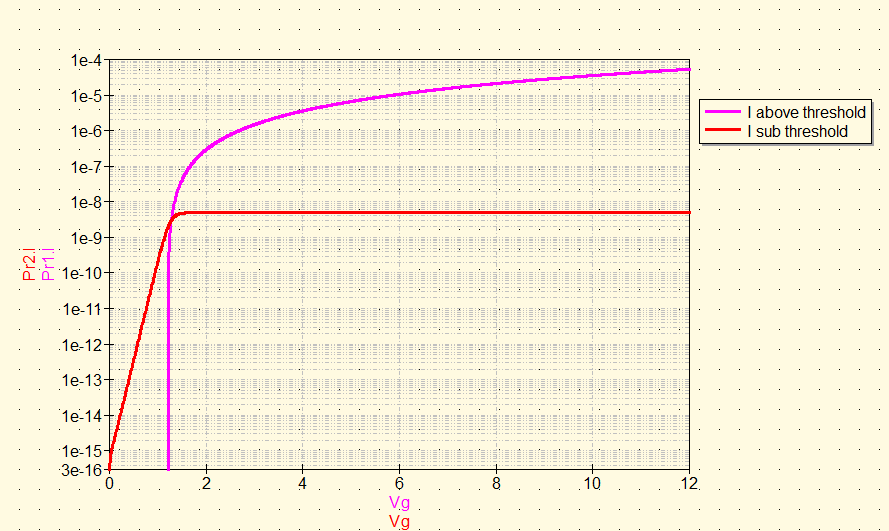
\includegraphics[scale = 0.6]{../Images/22072024/Ids-at-st.png}
\end{center}
\newpage
\subsection{Total current}
Total current $I_{DS}$ is given by addition of sub-threshold and above-threshold currents as shown in figure(\ref{fig:Itot})
\begin{center}
    \label{fig:Itot}
    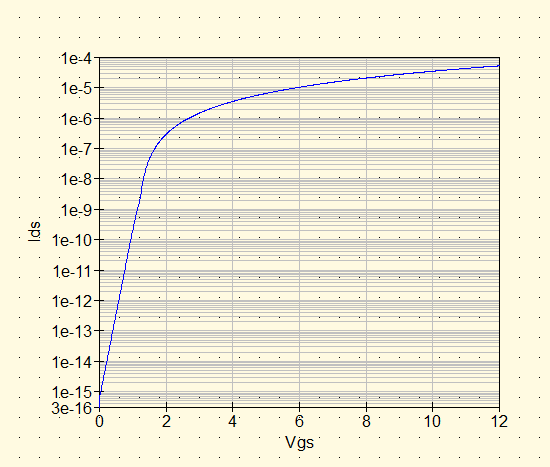
\includegraphics[scale=1]{../Images/22072024/Ids-total.png}
\end{center}

The sub-threshold and above threshold currents are added at a point  $V_{gs} = V_{th}+3V_T$ therefore, the slopes are not matched at that point. The gradient of the sub-threshold curve from the plot in the reference is found to be around 6.57 which should be equal to our $\frac{1}{m V_T}$ and that gives the value of $m = 5.85$. 

\hl{\textbf{To match the slope we need to find the gradients of each point on $I_{at}$ curve and find the point of $V_{gs}$ at which slope of $I_{at}$ is equal to slope of $I_{st} = 6.57$.  }}

\hl{\textbf{Currently, I am figuring out how to find the gradients at every point and check if the slope is equal to 6.57 using verilog A. I have found a python interfacing for qucs at https://github.com/zonca/python-qucs.git and trying to send find gradients using it. }}


\end{document}